\documentclass[
    left=2.5cm,         % Sadly, generic margin parameter
    right=2.5cm,        % doesnt't work, as it is
    top=2.5cm,          % superseded by more specific
    bottom=3cm,         % left...bottom parameters.
    bindingoffset=6mm,  % Optional binding offset.
    nohyphenation=false % You may turn off hyphenation, if don't like. 
]{eiti/eiti-thesis}

\usepackage[polish]{babel}
\usepackage[
    backend=bibtex,
    style=ieee
]{biblatex}
\usepackage{csquotes}
\usepackage{siunitx}

\usepackage{algorithm}
\usepackage[noend]{algorithmic}
\usepackage{graphicx}
\usepackage{cancel}
\usepackage{hyperref}


\newenvironment{polishalgorithm}[1][]
  {\begin{algorithm}[#1]
     \selectlanguage{polish}%
     \floatname{algorithm}{Algorytm}%
     \renewcommand{\algorithmicif}{\textbf{If}}%
     \renewcommand{\algorithmicthen}{\textbf{then}}%
     \renewcommand{\algorithmicend}{\textbf{end}}%
  }
  {\end{algorithm}}


\newcommand{\mycaptionof}[2]{\captionof{#1}{#2}}


\newcolumntype{H}{>{\setbox0=\hbox\bgroup}c<{\egroup}@{}}

\newcommand{\noaistats}[1]{}  %

% \definecolor{darkgreen}{rgb}{0,0.4,0.0}
% \definecolor{darkblue}{rgb}{0,0.1,0.3}
% \definecolor{darkred}{rgb}{0.7,0.0,0.0}

\newcommand{\lbs}{\ensuremath{B}}      %
\newcommand{\all}{\infty}
\newcommand{\lepochs}{\ensuremath{E}}  %
\newcommand{\clientfrac}{\ensuremath{C}}    %
\newcommand{\tnn}{2NN\xspace} %
\newcommand{\xx}{\hspace{-0.01in}\ensuremath{\times}}
\newcommand{\loss}{\ell}
\newcommand{\SUB}[1]{\ENSURE{} \hspace{-0.15in} \textbf{#1}}
\newcommand{\algfont}[1]{\texttt{#1}}

\renewcommand{\algorithmicensure}{}

\newcommand{\fedavglong}{\algfont{FederatedAveraging}\xspace}
\newcommand{\fedavg}{\algfont{FedAvg}\xspace}
\newcommand{\fedavgshort}{\algfont{FedAvg}\xspace}

\newcommand{\fedsgdlong}{\algfont{FederatedSGD}\xspace}
\newcommand{\fedsgd}{\algfont{FedSGD}\xspace}
\newcommand{\fedsgdshort}{\algfont{FedSGD}\xspace}

\newcommand{\eqdef}{\overset{\text{def}}{=}}
\newcommand{\T}{\rule{0pt}{2.2ex}}
\newcommand{\targetTNN}{97\%\xspace}
\newcommand{\targetCNN}{99\%\xspace}
\newcommand{\targetLSTM}{54\%\xspace}
\newcommand{\nc}{K}
\newcommand{\pp}{\mathcal{P}}


\newlength{\pw}


\newcommand{\BO}{\mathcal{O}}
\newcommand{\R}{\ensuremath{\mathbb{R}}}
\newcommand{\qqand}{\qquad \text{and} \qquad}
\newcommand{\qqwhere}{\qquad \text{where} \qquad}
\newcommand{\qqwith}{\qquad \text{with} \qquad}
\DeclareMathOperator*{\E}{\mathbb{E}}
\newcommand{\grad}{\triangledown}
\newcommand{\h}{\frac{1}{2}}




\graphicspath{{img/}}             % Katalog z obrazkami.
\addbibresource{bibliografia.bib} % Plik .bib z bibliografią

%----------------------------------------
% Twierdzenia i definicje;
% tutaj ew. tłumaczymy te terminy
% na inne języki
%----------------------------------------
\newtheorem{theorem}{Twierdzenie}
\newtheorem{lemma}{Lemat}
\newtheorem{corollary}{Wniosek}
\newtheorem{definition}{Definicja}
\newtheorem{axiom}{Aksjomat}
\newtheorem{assumption}{Założenie}




%----------------------------------------
% Spis rysunków, tablic i załączników;
% tutaj ew. tłumaczymy te terminy
% na inne języki
%----------------------------------------
\AtBeginDocument{
    \renewcommand{\listfigurename}{Spis rysunków}
    \renewcommand{\listtablename}{Spis tabel}
    \renewcommand{\tablename}{Tabela}
}

\begin{document}

% \renewcommand{\ALG@name}{Algorytm}

%--------------------------------------
% Strona tytułowa
%--------------------------------------
\EngineerThesis{} % dla pracy inżynierskiej mamy \EngineerThesis
\instytut{Automatyki i Informatyki Stosowanej}
\kierunek{Automatyka i Robotyka}

\title{
     System rozproszonej i bezpiecznej identyfikacji użytkownika urządzenia Internetu Rzeczy
}
\engtitle{ % Tytuł po angielsku do angielskiego streszczenia
    System for distributed and secure identification for the user of IoT device
}

\author{Dawid Kiciński}
\album{277115}
\promotor{mgr Maciej Stefańczyk}
\date{\the\year}
% \maketitle

%--------------------------------------
% Streszczenie po polsku
%--------------------------------------
% \streszczenie \lipsum[1-3]
% \slowakluczowe XXX, XXX, XXX
% \newpage

%--------------------------------------
% Streszczenie po angielsku
%--------------------------------------
% \abstract \kant[1-3]
% \keywords XXX, XXX, XXX
% \newpage

%--------------------------------------
% Oświadczenie o autorstwie
%--------------------------------------
% \makeauthorship
% \blankpage

%--------------------------------------
% Spis treści
%--------------------------------------
\thispagestyle{empty}
\tableofcontents
\blankpage{}

%--------------------------------------
% Rozdziały
%--------------------------------------

\newpage

\newpage
\section{Wstęp}

Coraz częściej urządzenia internetu rzeczy stają się głównymi urządzeniami komputerowymi coraz
większej liczby użytkowników~\cite{SmartphoneOwenrship,SmartphoneOwenrshipv2}. Często gromadzą one wrażliwe dane i dostęp do takich
urządzeń przez niewłaściwe osoby grozi nieodwracalnymi stratami dla ich właściciela. Nowe
przyrządy wyposażone w odpowiednie sensory pozwalają na uwierzytelnienie dostępu już nie tylko za
pomocą hasła ale również przez weryfikacje biometryczną. Zabezpieczenia biometryczne mogą się
opierać na rozpoznawaniu linii papilarnych, głosu, skanowaniu żył, czy też tęczówki lub siatkówki
oka. W szczególności popularnym rozwiązaniem jest weryfikacja użytkownika przez biometrie twarzy ~\cite{FaceBiometic}.

Metody weryfikacji twarzy (ją jakieś) wymagają wyspecjalizowanych i dokładnych kamer (need fact
check). Z jednej strony montowanie drogich i nowoczesnych kamer na urządzeniach IoT do celów
weryfikacji jest nieopłacalne finansowo, a z drugiej z perspektywy użytkownika pożądane jest
posiadanie możliwie dokładnego systemu weryfikacji dostępu. Najnowocześniejsze i najbardziej
dokładne metody bazują w całości lub przynajmniej części na bazie sieci neuronowych (cite,fact
check). Metody te pewnym stopniu niwelują potrzebę posiadania wyspecjalizowanych kamer jednak
dokładność nowoczesnych metod jest bardzo uzależniona od jakości i ilość danych, które posłużyły
do wytrenowania sieci neuronowej.

Sensory, w które wyposażone są te urządzania (aparat, mikrofon, itp), w połączeniu z
faktem, że są używane codziennie, gromadzą niebywałą ilość, zazwyczaj prywatnych,
danych. Modele wyuczone na takich danych dają znakomitą poprawę ich użyteczności jednak ze względu
na ich wrażliwy charakter wiąże się to z ryzykiem i wysoką odpowiedzialnością ich
przechowywania w scentralizowanej lokalizacji albo nawet całkowitym brakiem dostępu do tych
danych.

Federated Learning pozwala na bezpieczne dla użytkownika wykorzystanie jego prywatnych danych
w celu dotrenowania sieci neuronowych i w tym poprawy ich jakości. W tej pracy zostanie
zbadana metoda ta metoda uczenia sieci neuronowych w implementacji systemu rozpoznawania twarzy
systemu na urządzania IoT.

\smallbreak

Praca została podzielona na rozdziały. W rozdziale~\ref{sec:general} został przedstawiony ogólny
zarys implementowanego systemu. Opisujemy czym charakteryzują się urządzania IoT się, na czym
polega zadanie weryfikacji użytkownika i pokazujemy, że zastosowanie podejścia Federated
Learningu do tego zadania jest odpowiednie. Następnie w rozdziale~\ref{sec:verification} w
szczegółach zostaje opisany problem weryfikacji użytkownika na podstawie cech biometrycznych jego
twarzy. Omawiane zostają dwa współczesne podejścia wykorzystujące głębokie sieci neuronowe, ich
wady i zalety względem wykorzystania w FL. Prezentujemy dokładniej wybrane przez nas podejście
wraz z naszą implementacją i otrzymanymi wynikami. Rozdział~\ref{sec:federated} został poświęcony
na omówienie Federated Learningu. Opisujemy cechy środowiska, w którym zastosowanie tej metody
treningu sieci daje największy zysk, prezentujemy projekt całego systemu zaczynając od protokołu
komunikacji, założeń co do urządzeń końcowych oraz serwera. Omawiamy algorytm Federated
Averaging oraz jego implementacje. Ostatecznie w rozdziale~\ref{sec:fedfaceid}prezentujemy zastosowanie FL do dotrenowania
ekstraktora cech w rozproszonym zbiorze danych. Na końcu w rozdziale~\ref{sec:summary} zostało
zawarte podsumowanie tej pracy wraz z propozycją jej dalszego rozwoju.

\newpage
\section[general]{Modele neuronowe, a urządzenia końcowe}\label{sec:general}

Tworzenie modeli predykcyjnych typu sieć neuronowa opiera się na odpowiednim ustaleniu wag
wybranej architektury sieci. Taki model jest parametryzowany wagami - liczbami
zmiennoprzecinkowymi, które na podstawie przykładów trenujących są iteracyjnie poprawione przez
wybrany algorytm optymalizacji. Proces ten nazywany w literaturze jest treningiem. Po wytrenowaniu model trafia do środowiska produkcyjnego, w którym będzie dawał predykcje.

Przekazanie modelu do wykorzystania dla użytkowników można zrealizować na kilka sposobów. Sposób w jaki jest to wykonywanie zależy w dużej mierze od architektury środowiska produkcyjnego oraz typu urządzeń z jakich będą korzystali użytkownicy. W ramach wstępu do tematyki tej pracy uwaga zostanie zwrócona na właśnie te dwa zagadnienia.

% Federated Learning jest naturalną kontynuacją ostatnich trendów w dziedzinie treningu i deploymentu modeli neuronowych do środowisk produkcyjnych dlatego na wstępnie zostaną przedstawione typo
\subsection{Urządzenia IoT}

Istnieją rządzenia, którą komunikują się między sobą przez sieć internet. Mogą to być smartphone,
inteligentne zamki. Urządzenia są w jakiś sposób chronione przed dostępem osób nie autoryzowanych.

Wypunktować cechy charakterystyczne urządzeń IoT.
\subsection{Uwierzytelnienie użytkownika biometrią twarzy}

Tymczasem wiele rodzajów uwierzytelniania jest wadliwych, zwłaszcza hasła. Ponieważ przeciętny człowiek musi śledzić wiele haseł, z których wiele może wymagać regularnej aktualizacji, hasło stało się niepraktyczne i niepewne.

Przestępcy mogą „wyłudzić” ludzi z ich haseł. Lub mogą użyć oprogramowania „brute force”, aby
wypróbować miliony kombinacji słów co sekundę. Problem polega na tym, że obecnie nie istnieje
szeroko rozpowszechniona, uniwersalna (i wygodna) forma tożsamości cyfrowej. Odpowiedzią na to
może być uwierzytelnienie biometrią twarzy:

\begin{itemize}
    \item Jest nieinwazyjny, ponieważ użytkownik nie wymaga fizycznej interakcji
    \item Jest stosunkowo łatwy do wdrożenia i wdrożenia
    \item Koszty technologii - kamery, przetwarzanie - spadają
    \item Masowa adopcja przez producentów smartfonów sprawiła, że stało się to znane użytkownikom
    \item Jego wyniki są dokładne i szybkie
\end{itemize}

Z tego powodu twórcy smartfonów i tabletów używają teraz identyfikacji twarzy jako domyślnej metody „odblokowania” dla swoich urządzeń i usług. Rzeczywiście, Counterpoint Research spodziewa się, że w 2020 r. Pojawi się ponad miliard smartfonów z rozpoznawaniem twarzy.

Dzięki ulepszeniom technologii aparatu, procesom mapowania, uczeniu maszynowemu i szybkościom przetwarzania, rozpoznawanie twarzy z biegiem lat.

Większość systemów wykorzystuje technologię kamery 2D, która tworzy płaski obraz twarzy i mapuje „punkty węzłowe” (rozmiar / kształt oczu, nosa, kości policzkowych itp.). Następnie system oblicza względną pozycję węzłów i przekształca dane w kod numeryczny. Algorytmy rozpoznawania przeszukują zapisaną bazę danych twarzy w celu znalezienia dopasowania.

Technologia 2D działa dobrze w stabilnych, dobrze oświetlonych warunkach, takich jak kontrola paszportowa. Ale jest mniej skuteczny w ciemniejszych przestrzeniach i nie może zapewnić dobrych rezultatów, gdy obiekty się poruszają. Zdjęcie jest łatwe do sfałszowania.

Dzisiaj wcześniej zaawansowane procesy trafiają do urządzeń na rynku masowym. Na przykład, Apple wykorzystuje technologię kamery 3D do zasilania funkcji Face ID opartej na podczerwieni w swoim iPhonie X. Zdjęcia termiczne IR odwzorowują wzory twarzy pochodzące głównie ze wzoru powierzchownych naczyń krwionośnych pod skórą.
 
Kolejnym kluczowym postępem jest „głęboka splotowa sieć neuronowa”. Jest to rodzaj uczenia maszynowego, w którym model znajduje wzorce w danych obrazu. Wykorzystuje sieć sztucznych neuronów, które imitują funkcjonowanie ludzkiego mózgu. W efekcie sieć zachowuje się jak czarna skrzynka. Podano wartości wejściowe, których wyniki nie są jeszcze znane. Następnie sprawdza, czy sieć przynosi oczekiwany wynik. Gdy tak nie jest, system dokonuje regulacji, dopóki nie zostanie poprawnie skonfigurowany i będzie w stanie systematycznie generować oczekiwane wyniki.
\subsection{Wdrażanie modeli neuronowych na urządzenia końcowe}

Popularnym i prostym w implementacji środowiskiem produkcyjnym jest wdrożenie modelu w postaci
serwisu chmurowego~\cite{ServerFacebook}. Serwis postawiony na serwerze wystawia dla konsumentów
swoje sieciowe API. Na zapytanie o predykcje dla danych wejściowych serwer odsyła wyjście
zwrócone przez model - rysunek~\ref{fig:deploy-0}. Rozwiązanie to oczywistą zaletę - inferencja
modelu wykonywana jest w chmurze przez co urządzenie użytkownika nie zużywa swoich zasobów obliczeniowych oszczędzając energię oraz pamięć, jednak kosztem wymagania stałego dostępu urządzenia do internetu oraz potrzebą wysłania danych wejściowych do serwera.

\begin{figure}[h!]
    \centering
    \includegraphics[width=0.8\linewidth]{img/ml_server_0_drawio.pdf}
    \caption{Środowisko produkcyjne z serwisem chmurowym.}
    \label{fig:deploy-0}
    \vspace{-4mm}
\end{figure}

Innym, coraz to bardziej popularnym, podejściem jest wdrożenie modeli bezpośrednio na urządzenia
końcowe~\cite{EdgeFacebook}(rysunek~\ref{fig:deploy-1}). Jest to proces o tyle bardziej
skomplikowany przez to, że aktualnie popularne frameworki\cite{PyTorch,Tensorflow,Mxnet} do
budowania i trenowania sieci neuronowych nie wspierają większości platform, na których budowane
są urządzenia IoT. Taki sposób wdrożenia modelu pozwala na korzystanie z modelu w trybie offline,
zwalnia nas z obowiązku utrzymywania serwera produkcyjnego oraz nie zmusza użytkownika do
wysyłania danych na zewnątrz urządzenia. Niestety narzucamy przez to duże ograniczenia na model
oraz na docelowe urządzenie IoT. Urządzenia końcowe mają o wiele niższe możliwości obliczeniowe
oraz pamięciowe dlatego wdrażany model powinien być dostatecznie mały tak aby zbytnio nie
obciążać urządzenia. Aktualnie urządzenia zdolne do uruchomienia sieci wyprodukowanych przez
popularniejsze frameworki to wszystkie platformy obsługujące system linux oraz smarfony z
systemem Android lub iOS.

\begin{figure}[h!]
    \centering
    \includegraphics[width=0.5\linewidth]{img/ml_server_1_drawio.pdf}
    \caption{Środowisko produkcyjnego - wdrożenie modelu bezpośrednio na urządzenia końcowe.}
    \label{fig:deploy-1}
    \vspace{-4mm}
\end{figure}

Na rysunku~\ref{fig:deploy-2} przedstawiono schematyczne dotrenowanie modeli na urządzeniach
końcowych na danych znajdujących sie na urządzeniach. Wykorzystujemy w ten sposób zbierane przez
urządzenia dane i aktualizujemy wagi modelu wykorzystując dane pochodzące bezpośrednio od
użytkownika. Urządzenie zyskuje w ten sposób model
lepiej spersonalizowany pod swoją dystrybucje danych wejściowych. Modele nie są współdzielone,
każdy z użytkowników ma swóją wersje modelu.

\begin{figure}[h!]
    \centering
    \includegraphics[width=0.8\linewidth]{img/ml_server_2_drawio.pdf}
    \caption{Wdrożenie na urządzenia końcowe i dotrenowanie modelu wykorzystując lokalnie zbierane dane}
    \label{fig:deploy-2}
    \vspace{-4mm}
\end{figure}

Na rysunku~\ref{fig:deploy-3} przedstawione zostało podejście Federated Learningu. Od poprzednika
różni go tylko element serwera FL, który pobiera dotrenowane modele od urządzeń agreguje je i
rozsyła je z powrotem. Podejście to pozwala na lepszą generalizacje modeli i w efekcie lepszą
predykcję. Niestety przez wprowadzenie serwera pośredniczącego w wymianie modeli cały system
ulega znacznemu skomplikowaniu i wymagany jest odpowiedni protokół dotrenownywania, agregacji i
wymiany modeli. W szczegółach to podejście zostanie omówione w rozdziale~\ref{sec:federated}.

\begin{figure}[h!]
    \centering
    \includegraphics[width=1\linewidth]{img/ml_server_3_drawio.pdf}
    \caption{Wdrożenie modelu i dalsze jego dotrenowywanie stosując podejście Federated Learning}
    \label{fig:deploy-3}
    \vspace{-4mm}
\end{figure}


% User verification
% - Biometria twarzy
% - Ogólna procedura weryfikacji 
% - Przetwarzanie wstępne 
% - Neuronowy extractor cech
%   * Klasyfikacja
%   * Triplet loss
%       - Negative examples sampling
% - Implementacja


\section[verification]{System weryfikacji użytkownika za pomocą biometrii twarzy}\label{sec:verification}
\subsection{Komercyjne systemy weryfikacji twarzy}

\subsection{Procedura weryfikacji przy wykorzystaniu sieci neuronowych} 

Weryfikacja twarzy jest zadaniem przyrównania twarzy kandydata 
do innej i sprawdzenie czy nastąpiło ich dopasowanie. Jest to mapowanie
jeden-do-jednego: należy sprawdzić czy jest to ta sama osoba.

Mając na wejściu systemu dwa zdjęcia \(x_i\) oraz \(x_j\) wynik weryfikacji będzie wyznaczany następująco:

\begin{align}\label{eq:ekstraktor_weryfikacja}
\text{weryfikacja jest}\begin{cases}
    \text{pozytywna},& \text{jeśli } d(f(x_i), f(x_j) < \alpha \\
    \text{negatywna},              & \text{w.p.p}
\end{cases}
\end{align}

gdzie \(f(x)\) jest wektorem cech obrazu \(x\), opisanym w sekcji
\ref{sec:ekstraktor}, \(\alpha\) jest marginesem, \(d(f_1, f_2)\) jest pewną funkcją dystansu liczoną pomiędzy wektorami wyznaczanymi przez \(f(x)\).

\subsection{Wstępne przetwarzanie obrazu}
\subsubsection{Normalizacja obrazu}

\subsubsection{Normalizacja pozy}

\begin{figure}[H]
    \begin{center}
    \renewcommand\tabcolsep{1pt}
    {\bf Poprawna detekcja}
    \begin{tabular}{cc||cc||cc}
      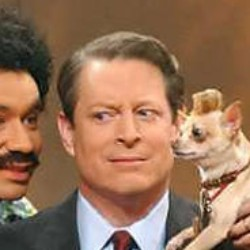
\includegraphics[width=.15\linewidth]{img/crop_examples/before/good/Al_Gore_0007.jpg} &
      
\includegraphics[width=.15\linewidth]{img/crop_examples/after/good/Al_Gore_0007.jpg} &
      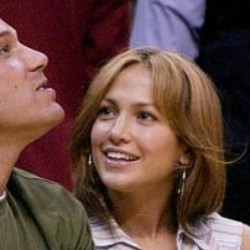
\includegraphics[width=.15\linewidth]{img/crop_examples/before/good/Jennifer_Lopez_0021.jpg} &
      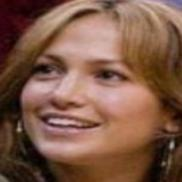
\includegraphics[width=.15\linewidth]{img/crop_examples/after/good/Jennifer_Lopez_0021.jpg} &
      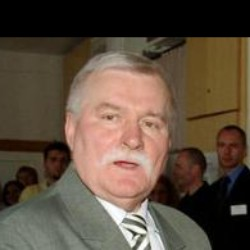
\includegraphics[width=.15\linewidth]{img/crop_examples/before/good/Lech_Walesa_0002.jpg} &
      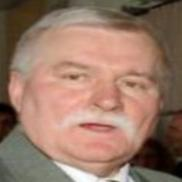
\includegraphics[width=.15\linewidth]{img/crop_examples/after/good/Lech_Walesa_0002.jpg} \\
    \end{tabular}
    {\bf Niepoprawna detekcja}
    \begin{tabular}{cc||cc||cc}
      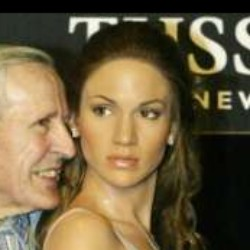
\includegraphics[width=.15\linewidth]{img/crop_examples/before/bad/Jennifer_Lopez_0020.jpg} &
      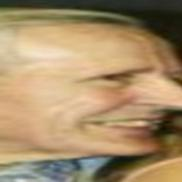
\includegraphics[width=.15\linewidth]{img/crop_examples/after/bad/Jennifer_Lopez_0020.jpg} &
      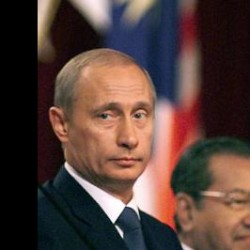
\includegraphics[width=.15\linewidth]{img/crop_examples/before/bad/Vladimir_Putin_0031.jpg} &
      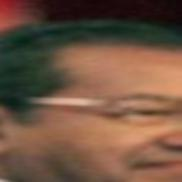
\includegraphics[width=.15\linewidth]{img/crop_examples/after/bad/Vladimir_Putin_0031.jpg} &
      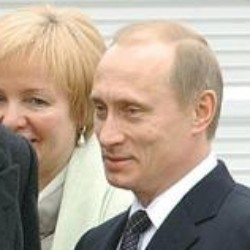
\includegraphics[width=.15\linewidth]{img/crop_examples/before/bad/Vladimir_Putin_0040.jpg} &
      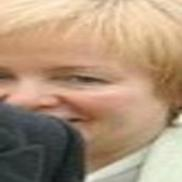
\includegraphics[width=.15\linewidth]{img/crop_examples/after/bad/Vladimir_Putin_0040.jpg} \\
    \end{tabular}
    \end{center}
    \caption{{\bf Przykłady działania ekstraktora twarzy.} Pokazane zostały tutaj wybrane przykłady prezentujące działanie ekstraktora twarzy.}
    \label{fig:ekstraktor_twarzy}
    \end{figure}

\subsection{Neuronowy ekstraktor cech} \label{sec:ekstraktor}
We współczesnych systemach weryfikacji wykorzystuje się głębokie sieci konwolucyjne. W
szczegółach zostaną omówione używana przez nas architektura w sekcji XXX. Pomijając szczegóły
modelu i traktując go jako czarną skrzynkę ogólna idea ekstraktora została pokazana na Rysunku
\ref{fig:ekstraktor_cech}. Głównym założeniem jest stworzenie systemu end-to-end, którego
rezultatem działania będzie embedding \(f(x)\), wyznaczony z obrazu wejściowego \(x\) przez
rzutowanie go do pewnej przestrzeni cech \(\mathbb{R}^d\), w taki sposób, że pewna funkcja
odległości wyznaczona dla wszystkich zdjęć twarzy jest mała dla twarzy należących do tych samych
osób i duża dla różnych twarzy. 

\begin{figure}[h]
    \centering
    \includegraphics[width=0.75\textwidth]{2-0_verification_ekstraktor_cech_drawio.pdf}
    \caption{\textbf{Struktura ekstraktora cech.} Ekstraktor składa się z wejścia, które w ogólnym przypadku może być paczką \(B\) przetworzonych wstępnie obrazów twarzy o wymiarach \( W \times H \times C\), głębokiej sieci konwolucyjnej i następującej po niej warstwie normalizacji. W rezultacie na wyjściu otrzymujemy \(B\) wektorów cech o wymiarach \(D\).}
    \label{fig:ekstraktor_cech}
\end{figure}


W literaturze można znaleźć dwie rodziny algorytmów trenujących, jedna wzorująca się na
klasycznym podejściu stosowanym podczas treningu klasyfikatorów obrazów. Najnowsze podejścia z
tej rodziny algorytmów prezentujemy w sekcji \ref{sec:klasyfikatory}. Drugi rodzaj algorytmów
bazują na optymalizacji multi-class classification hinge loss (po pl?). Opisujemy je w
szczegółach w sekcji \ref{sec:tripletloss}

\subsubsection{Klasyfikacja twarzy}\label{sec:klasyfikatory}
\begin{figure}[h!]
\centering
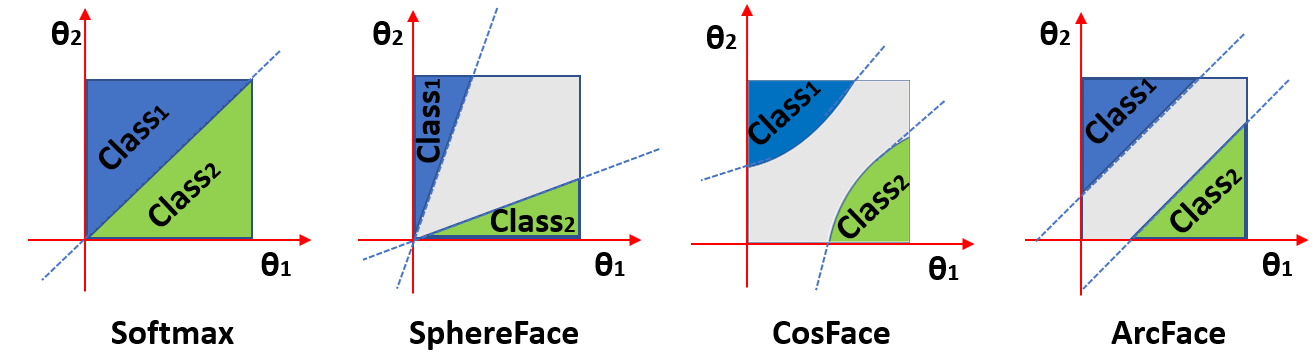
\includegraphics[width=1\linewidth]{img/margincompare.png}
\caption{Porównanie marginesów decyzyjnych\cite{}}
\vspace{-4mm}
\label{fig:binarymargin}
\end{figure}
\paragraph{Softmax\cite{Centreloss}}
\paragraph{SphereFace}
\paragraph{CosFace\cite{Cosface}}
\paragraph{ArcFace\cite{Arcface}}


\subsubsection{FaceNet}\label{sec:tripletloss}
% \begin{align}\label{eq:triplet_dystant}
    % \left\Vert f(x_i) - f(x_j) \right\Vert_q^p < \alpha
% \end{align}




%  Implementacja
% - datasets


\subsection{Trening ekstraktora cech FaceNet}
Niestety dużą wadą wybranego ekstraktora cech jest brak dobrej jakości implementacji oraz co gorsza  brak raportów skutecznego odtworzenia wyników prezentowanych przez autorów. Z tego względu w tej sekcji pracy zaprezentowana zostanie własna próba re-implementacji.

\paragraph{Szczegóły implementacji}
Wszystkie elementy procesu weryfikacji zostały zaimplementowane w języku Python z wykorzystaniem
frameworku PyTorch. Jako architekturę CNN wybrano popularny model ResNet-50. Głównie ze względu
na dużą moc reprezentacji oraz stabilny trening (Na tym etapie szybkość i wielkość modelu nie
była brana pod uwagę). Poza tym implementacja była jak najdokładniej odwzorowywana według 
zaleceń autorów zawartych w publikacji~\cite{Facenet}.
Niestety autorzy trenowali model na swoim prywatnym zbiorze danych o wielkości do 200 milionów
zdjęć pochodzących od 8 milionów osób. Niestety nie istnieją otwarte zbiory o podobnych
wielkościach.

\paragraph{Zbiory danych}
W literaturze znajduje się duża liczba zbiorów do treningu ekstraktorów cech twarzy.
Popularnym wyborem jest zbiór MS1M, posiada on duża różnorodność twarzy oraz duża liczbę
przykładów trenujących. VggFace2 jest relatywnie nowym zbiorem i nie tak popularnym jak poprzedni
ale cechuje się nie tylko dużym rozmiarem ale i dużą różnorodnością wewnątrz-klasową.

LFW jest jest niejako standardem w testowaniu systemów do weryfikacji, jednak ze względu na jego niewielkie rozmiary i niską różnorodność wewnątrz-klasową nie będzie odpowiedni do testowania systemu opartego o FL dlatego jego zastosowanie ograniczymy do walidacji pre-trenowanych  modeli trenowanych w tradycyjnym sposobem na serwerze.

W tabeli~\ref{table:dataset} znajduje sie podsumowanie wspomnianych wcześniej zbiorów danych .

\begin{table}[h]
\begin{center}
\begin{tabular}{c|c|c|c|c}
\hline
Zbiór danych  & \# osób   &   \# zdjęć  &   \# zdjęć na osobę (średnia)   &  wyrównane \\
\hline
VGGFace2-train \cite{DatasetVGGFace2}     & 9.1K & 3.3M & 362.6 & Nie  \\ 
MS1M-DeepGlint \cite{DatasetGlintweb}   & 87K  & 3.9M & 44.8 & Tak \\
\hline
%  Walidacja  & \# osób   &   \# zdjęć  &   \# zdjęć na osobę   &   aligned \\
\hline
LFW \cite{DatasetLFW}   & 5,749  & 13,233 & 2.3& Nie \\
\hline
\end{tabular}
\end{center}
\caption{\textbf{Zbiory danych}.}
\label{table:dataset}
\vspace{-4mm}
\end{table}

Ze względu na bardzo dobrą jakość i zróżnicowanie wewnątrz-klasowe do treningu sieci zostanie wykorzystany zbiór VggFace2. Przed prezentacją wyników  zostanie najpierw omówiona metodyka ewaluacyjna.

\paragraph{Ewaluacja}
Do ewaluacji będzie wykorzystany LFW. Ma on zdefiniowany zbiór
par zdjęć twarzy, które należy określić czy należą do jednej czy dwóch różnych osób.
Wszystkie pary \(i,j\) twarzy należących do jednej osoby niech będą oznaczone przez
\(\mathcal{P_\text{same}}\), z kolei wszystkie pary twarzy różnych osób będą oznaczone przez
\(\mathcal{P_\text{diff}}\).
Definiujemy zbiór wszystkich poprawie zaakceptowanych (\emph{true accept}) par jako 
\begin{equation}
    \ta(\alpha)=\{(i,j)\in\mathcal{P_\text{same}}, \quad \text{dla} \quad \,d(x_i,x_j)\leq \alpha\}\;.
\end{equation}
Zbiór ten zawiera wszystkie pary twarzy, które zostały poprawie zaklasyfikowane jako te same przy zastosowanym progu. Podobnie 
\begin{equation}
  \fa(\alpha)=\{(i,j)\in\mathcal{P_\text{diff}}, \quad \text{dla} \quad \,d(x_i,x_j)\leq \alpha\}
\end{equation}
jest zbiorem wszystkich par, które został nie poprawnie zaklasyfikowane jako te same (\emph{false accept}).
Definiujemy dwie metryki, \emph{true accept rate} \(\tar(\alpha)\) oraz \emph{falce accept rate} \(\far(\alpha)\), które dla danego progu \(\alpha\) wyznacza się jako
\begin{equation}
    \tar(\alpha)=\frac{\left|\ta(\alpha)\right|}{\left|\mathcal{P_\text{same}}\right|}\;,\quad
    \far(\alpha)=\frac{\left|\fa(\alpha)\right|}{\left|\mathcal{P_\text{diff}}\right|}\;.
\end{equation}
 Metryka, która będzie wykorzystywana do oceny jakości weryfikacji to stosowana we wzorcowym
 artykule \(\tar@\far=\num{0.001}\). Wyznacza się ją następująca: 1) stosując zbiór walidacyjny
 należy znaleźć taki próg \(\alpha\), dla którego \(\far(\alpha)\) wyniesie \(\num{0.001}\). 2)
 policzyć metrykę \(\tar(\alpha)\) dla wyznaczonego progu \(\alpha\).
  
\paragraph{Wyniki eksperymentów}

Ze względu na bardzo długi czas treningu i ograniczone zasoby sprzętowe udało się znaleźć tylko jeden zestaw paramtetrów, który pozwolił na względnie stabilną naukę modelu. Model trenowano  na karcie graficznej Nvidia RTX2070, skorzystano z szybkich operacji 16fp i trening trwał ponad 7 dni. Trenowany model był co kilka tysiecy kroków walidowany, co zostało zwizualizowane na rysunku~\ref{fig:facenet_train}.

\begin{figure}[h]
  \centering
  \includegraphics[width=0.70\textwidth]{img/facenet_train.pdf}
  \caption{\fedavglong}%
  \label{fig:facenet_train}%
\end{figure}

Niestety nie udało sie odtworzyć wyników raportowanych przez autorów, którzy osiągneli
\(\tar@\far=\num{0.001}\) wynoszący ponad \num{0.9}. Może to wynikać z
\begin{itemize}
    \item zbyt krótkiego czasu trenigu,
    \item braku zbliżonego wielkością zbioru danych użytych do uzyskania raportowanych wyników.
\end{itemize}

Jeśli spekulowane powody porażki są prawdziwe to przeprowadzony eksperyment można uznać za sukces
- implementacja jest poprawna, model się uczy jednak wymaga więcej czasu aby osiągnąć zbieżność.
Co oznacza, że można pójść krok dalej i spróbować dotrenować ekstraktor cech stosująć podejście
FL. Ze względu na wcześniej wspomniany brak dostępnych modeli FaceNet i braku możliwości
wytrenowania takiego modelu samodzielnie będziemy musieli zdecydować się na dotrenowywanie
innego, dostępnego, ekstraktora cech trenowanego inną metodą. Eksperymentowano z tym już w
\cite{Arcface}, gdzie wstępnie wytrenowano model metodą ArcFace i pod koniec dodatkowo
dotrenowano samą sieć CNN właśnie przy pomocy funkcji triple loss. Wyniki w
tabeli~\ref{table:losscompare} pokazują, że można osiągnąć tą techniką bardzo dobre rezultaty.

\subsection{Podsumowanie}
W tym rozdziale został omówiany proces weryfikacji, został wybrany detektor twarzy oraz
ekstraktor cech twarzy. Została podjęta próba implementacji wybranej metody wyznaczania
embeddingów, która zakończyła się w pewien sposób sukcesem - nie udało się odtworzyć
raportowanych wyników ale za to została pozytywnie zweryfikowana implementacja.

Eksperymenty przeprowadzane w ten sekcji zostaną kontunuowane dalej w rozdziale~\ref{sec:fedfaceid}. Jednak przed tym zostanie po krótce omówiona idea Federated Learningu.


%see this:
%https://arxiv.org/pdf/1901.08616.pdf
%https://arxiv.org/pdf/1709.02940.pdf




\newpage
\section[federated]{Federated Learning}\label{sec:federated}

W tym rozdziale przedstawiony zostanie projekt systemu, który korzystając z podejścia Federated  Learning (FL) umożliwi na trening ekstraktora cech twarzy w rozproszonym środowisku urządzeń IoT.


\paragraph{Federated Learning}

Federated Learning (FL) jest podejściem zastosowania uczenia maszynowego w rozproszonym
środowisku pozwalającym na trening na on dużym zbiorze zdecentralizowanych prywatnych
danych znajdujących się na urządzeniach końcowych użytkowników, a w szczególności urządzeniach
Internetu Rzeczy. FL realizuje ideę `przyniesienie kodu do danych, zamiast danych do kodu' i
adresuje fundamentalne problemy prywatności, własności i lokalności danych. Federated learning
został opisany w \cite{FLBasic,FLSystemDesign,FLOptimization,FLSecureAggregation}.
Problemy odpowiednie do zastosowania federated learningu mają następujące właściwości:
\begin{itemize}
  \item Trening na rzeczywistych danych gromadzonych na urządzaniach mobilnych daje znaczą przewagę
  nad treningiem na ogólnie dostępnych danych proxy dostępnych w centrach danych.
  \item Te dane są prywatne albo są zbyt duże do ich przechowywania.
  \item Dla zadań nadzorowanych, etykiety danych powstają samoistnie z interakcji użytkownika z urządzeniem.
\end{itemize}

\paragraph{Cechy środowiska systemu}

Algorytmy optymalizacji mogące być zastosowane do optymalizacji na urządzaniach IoT mają kilka cech wyróżniających je od znanych już algorytmów rozproszonej optymalizacji:
\begin{itemize}

\item \textbf{Non-IID} Dane trenujące na danym urządzaniu są zazwyczaj zależne od konkretnego użytkownika i dlatego lokalny zbiór danych zebrany na dowolnym urządzeniu nie będzie reprezentatywny w stosunku do dystrybucji całej populacji
\item \textbf{Niezbalansowany} Podobnie, niektórzy użytkownicy będą o wiele częściej korzystali z aplikacji aparatu niż inni, co będzie prowadziło do różnic w wielkości zebranych lokalnych zbiorów  danych trenujących.
\item \textbf{Masywnie rozproszony} Spodziewa się, że liczba finalnych użytkowników biorąca udział w optymalizacji będzie większa niż średnia liczba przykładów trenujących przypadająca na jednego klienta.
\item \textbf{Ograniczona komunikacja} Urządzania IoT mogą być ograniczone wolnym albo kosztownym łączem sieciowym.
\end{itemize}

W tej pracy główna uwaga zostanie poświęcona na doprowadzenie systemu do działania w patologicznym przypadku środowisku danych Non-IID oraz ograniczonej i zawodnej komunikacji.


\subsection{Projekt systemu}

Implementowany system umożliwia trening głębokich sieci neuronowych on danych bezpośrednio przetrzymywanych na
urządzaniu IoT. Dane te nigdy nie opuszczają samego urządzania. Wagi modeli użytkowników są
agregowane i łączone na serwerze znajdującym się w chmurze za pomocą algorytmu Federated
Averaging konstruując nowy model globalny, który zostaje przesłany z powrotem do urządzeń końcowych
do inferencji. System ten został opisany pierwotnie w \cite{FLBasic} i z sukcesem zaaplikowany w
implementacji inteligentnej klawiatury smartphone~\cite{FLBlog}.


Przedstawienie architektury systemu zaczynamy od przedstawienia protokołu według, którego przebiega cały przepływ danych.

\subsubsection{Protokół}

Uczestnikami protokołu są urządzania Internetu Rzeczy oraz serwer, który jest usługą chmurową.
Urządzania anonsują serwerowi swoją gotowość do uruchomienia zadania. Zadanie jest specyficzne dla populacji urządzeń i polega na lokalnym uruchomieniu obliczeń, takich jak trening z zadanymi przez serwer parametrami albo ewaluacja wytrenowanego modelu na lokalnych dla urządzenia danych.

Protokół dzieli komunikacje na rundy, z której każda zaczyna się od selekcji. Z potencjalnie tysięcy gotowych urządzeń w danym oknie czasowym, serwer wybiera ich podzbiór, który dostanie zaproszenia do wzięcia udziału obliczeniach. Liczebność tego podzbioru jest parametrem algorytmu opisywanego w kolejnym rozdziale

Serwer mówi wybranym urządzeniom jakiego typu obliczenia będą wykonywane. Wraz z tą informacją
przesyłany jest graf obliczeniowy modelu, zserializowane parametry globalnego modelu oraz pozostałe
informacje niezbędne do uruchomienia obliczeń w danej rundzie. Następnie każdy z uczestników  wykonuje lokalnie obliczenia bazując na globalnym stanie oraz swoim lokalnym zbiorze danych i przesyła wynik obliczeń z powrotem na serwer. W szczególności wynikiem, w przypadku rundy treningowej, będą wytrenowane parametry modelu lokalnego. Serwer wciela zebrane aktualizacje w swój stan globalny co kończy pojedyńczą rundę i proces ten się powtarza.

Opisywany protokół pozwala urządzeniom końcowym na poprawianie globalnego, pojedyńczego modelu pomiędzy rundami, z których każda składa się z trzech faz: selekcji, konfiguracji oraz raportowania.

\paragraph{Selekcja}
Cyklicznie, urządzenia, które spełniają wymagane kryteria meldują serwerowi swoją gotowość. Serwer wybiera podzbiór z dostępnych mu urządzeń. W naszej implementacji wybrano prostą, losową selekcje  z rozkładem jednostajnym \(N\) urządzeń z tych, które
ogłosiły swoją gotowość. 


\paragraph{Konfiguracja}
Serwer jest skonfigurowany na podstawie wybranego mechanizmu selekcji urządzeń oraz agregacji
modeli. Urządzenia końcowe są samo-konfigurowane według przesłanej przez serwer informacji o typie obliczeń, grafu obliczeniowego oraz stanu globalnego.

\paragraph{Raportowanie}
Serwer czeka, aż partycypujące urządzenia zdadzą raport z wynikiem przeprowadzonych obliczeń. Jeśli runda była rundą treningową to wraz z otrzymaniem wszystkich zaktualizowanych modeli, serwer agreguje je z użyciem algorytmu Federated Averaging i informuje raportujące urządzenia kiedy mogą ponownie zgłosić swoją gotowość. Jeśli wystarczająca liczba urządzeń zaraportuje wyniki serwerowi w pewnym oknie czasowym, runda zostanie uznana za zakończoną z powodzeniem i zagregowany model zastąpi aktualny model globalny. W przeciwnym przypadku zebrane wyniki z tej rundy zostają porzucone. Protokół jest w pewnym stopniu odporny na to, że partycypujące urządzenia z pewnych powodów nie odpowiedzą na przesłaną konfiguracje albo nie zaraportują wyników.

\vspace{5mm}

Fazy selekcji i raportowania są dospecyfikowane przez zestaw parametrów. Podczas fazy selekcji  serwer bierze pod uwagę pożądaną liczbę uczestników rundy, czasy time-outów oraz minimalną liczbę potrzebnych uczestników do rozpoczęcia rundy. Faza selekcji trwa dopóty dopóki nie zostanie wybrana docelowa liczba urządzeń albo nie skończy się czas przeznaczony na faze selekcji. W drugim przypadku runda zostanie rozpoczęta jeśli została zebrana minimalna liczba urządzeń, w przeciwnym przypadku runda zostaje porzucona. Faza raportowania parametryzowana jest przez minimalną liczbę urządzeń, które muszą zaraportować wynik.


\subsection{Algorytm optymalizacji}
  Algorytm \fedavglong~\cite{FLBasic}~\ref{alg:fedavg} opisany został zaimplementowany w języku Python. Do implementacji modeli
  neuronowych i algorytmów uczących został wykorzystany framework
  PyTorch~\cite{PyTorch}. Poprawność implementacji została sprawdzona w sekcji \ref{implementacja_fl} na zadaniu klasyfikacji obrazów wykorzystując prostą sieć konwolucyjną oraz popularny zbiór danych CIFAR10. 
  \begin{polishalgorithm}[t]

    \begin{algorithmic}
    \SUB{Serwer wykonuje:}
      \STATE{} initialize $w_0$
      \FOR{each round $t = 1, 2, \dots$}
        \STATE{} $m \leftarrow \max(\clientfrac\cdot K, 1)$
        \STATE{} $S_t \leftarrow$ (random set of $m$ clients)
        \FOR{each client $k \in S_t$ \textbf{in parallel}}
          \STATE{} $w_{t+1}^k \leftarrow \text{ClientUpdate}(k, w_t)$ 
        \ENDFOR{}
        \STATE{} $w_{t+1} \leftarrow \sum_{k=1}^\nc \frac{n_k}{n} w_{t+1}^k$
      \ENDFOR{}
      \STATE{}
    
    \SUB{ClientUpdate ($k, w$):}\ \ \  // \emph{Run on client $k$}
      \STATE{} $\mathcal{B} \leftarrow$ (split $\pp_k$ into batches of size $\lbs$)
      \FOR{each local epoch $i$ from $1$ to $\lepochs$}
        \FOR{batch $b \in \mathcal{B}$}
          \STATE{} $w \leftarrow w - \eta \grad \loss(w; b)$
        \ENDFOR{}
    \ENDFOR{}
    \STATE{} return $w$ to server
    \end{algorithmic}
    \mycaptionof{algorithm}{\fedavglong. The $\nc$
      clients are indexed by $k$; $\lbs$ is the local minibatch size,
      $\lepochs$ is the number of local epochs, and $\eta$ is the learning
      rate.}\label{alg:fedavg}
    \end{polishalgorithm}



  \subsection{Implementacja optymalizacji FL}\label{implementacja_fl}
  \subsubsection{Sieć konwolucyjna}

  Jako obiekt treningu omawianego algorytmu zastała użyta niewielka sieć neuronowa zawierająca
  dwie warstwy konwolucyjne z filtrami o szerokości 5x5 (pierwsza z 32 kanałami, druga z 64, po
  każdej dodatkowa warstwa 2x2 max pooling), po których następuje dwu-warstwowy perceptron i na
  końcu warstwa przekształcenia liniowego, co daje w sumie \(10^6\) milionów parametrów. Model został podsumowany w tabeli 


  \subsubsection{Zbiory danych}
  \paragraph{CIFAR10}
  CIFAR10 jest popularnym syntetycznym zbiorem danych. Zbiór danych składa się z \(\num{60000}\)
  kolorowych obrazów podzielonych na \(\num{10}\) klas, z \(\num{6000}\) obrazami przypadającymi
  na jedną klasę. Zawarte są w nim obrazy o szerokości i wysokości 32 pikseli. Standardowo zbiór
  dzieli się na dwa zbalansowane klasowo podzbiory: testowy i treningowy zawierających odpowiednio
  \(10000\) i \(50000\) etykietowanych przykładów. Na rysunku~\ref{fig:cifar10_example} znajduje się 10 losowo wybranych obrazów, dla każdej z 10 klas.

  \begin{figure}[h]
    \centering
    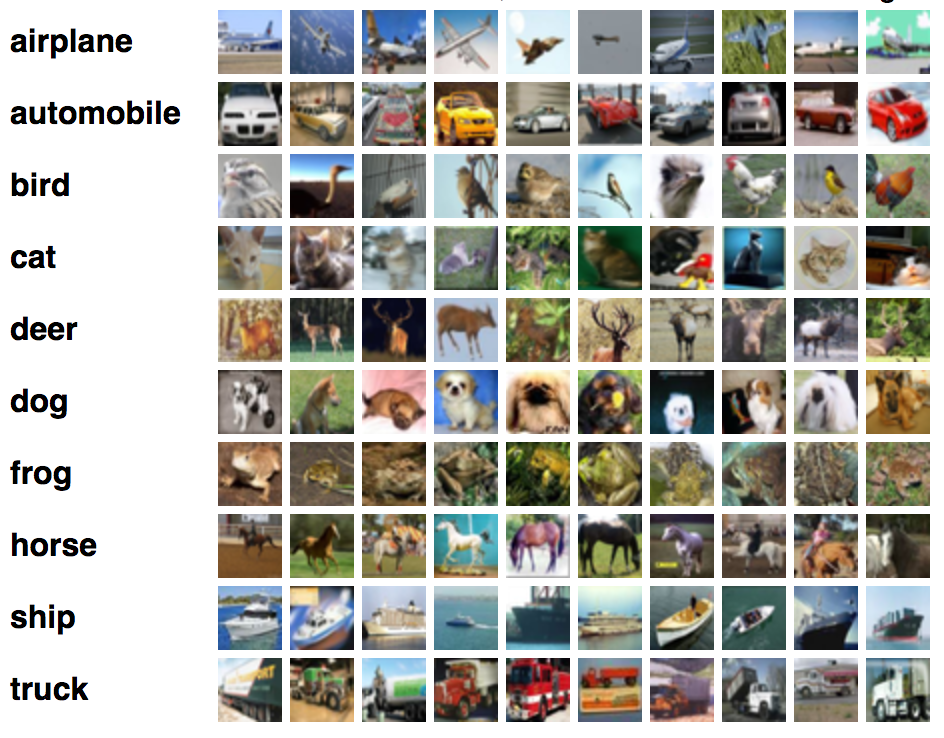
\includegraphics[width=1.0\textwidth]{img/cifar10_example.png}
    \mycaptionof{figure}{10 przykładowych obrazów dla każdej z \(\num{10}\) klas zbioru CIFAR10}
    \label{fig:cifar10_example}
  \end{figure}

  \subsubsection{Protokół treningowy}

  Do sprawdzenia poprawności implementacji została zaimplementowana procedura treningowa wzorowana
  na~\cite{FLBasic}. Zbiór treningowy został podzielony pomiędzy 100 użytkowników tak żeby każdy zawierał po 500 przykładów trenujących. Z powodu braku naturalnego podziału danych na tak dużą liczbę klientów rozważany jest tutaj nieco mniej wymagający przypadek, w którym dane każdego użytkowania są zbalansowane oraz równomiernie rozdystrybuowane.

  Naszym celem była maksymalizacja dokładności z jaką model klasyfikował obrazy pochodzące ze
  zbioru testowego. Badanie jakości końcowego modelu globalnego odbywało się już nie w sposób
  rozproszony, a na serwerze stosując cały dostępny zbiór testowy, co zostało umożliwione dzięki wprowadzonym uproszczeniom co do rozkładu danych.

  Obrazy uległy standardowemu przetworzeniu wstępnemu i augmentacji. Przykłady trenujące zredukowano do wielkości 24x24 pikseli przez losowe obcięcie krawędzi, obrazy uległy losowemu horyzontalnemu odbiciu lustrzanemu  oraz standardowej normalizacji.

  Zaimplementowany algorytm został porównany do standardowego algorytmu SGD~\cite{SGD}.


  \subsubsection{Ewaluacja}
% \newcommand{\acc}[1]{\multicolumn{2}{c}{#1\%}}
\begin{table}[h]\label{table:cifar}
  \begin{center}
  \begin{tabular}{ccc}
    \hline
    Acc.     &   80\%  & 82\% \\
    \hline
    \algfont{SGD}  & 18000  & 31000 \\
    \fedavg     &   280~(64.3\xx) & 630~(49.2\xx) \\
    \hline
    \algfont{SGD}~re-implementacja  & 20500 & 45000 \\
    \fedavg~re-implementacja    &   510~(40.2\xx) & 1200~(37.5\xx) \\
    \hline
  \end{tabular}
\end{center}
  \mycaptionof{table}{Liczba aktualizacji modelu globalnego i przyspieszenie względem podstawowego SGD potrzebna do otrzymania zadanej dokładności (Acc) na testowym zbiorze CIFAR10.}
\end{table}

\begin{figure}[h]
  \centering
  \includegraphics[width=0.60\textwidth]{img/baseline.pdf}
  \caption{\algfont{SGD}}%
  \label{fig:baseline}%
\end{figure}

\begin{figure}[h]
  \centering
  \includegraphics[width=0.60\textwidth]{img/fed_avg.pdf}
  \caption{\fedavglong}%
  \label{fig:fedavg}%
\end{figure}

  \section{Protokołu treningowy FL do zadania weryfikacji twarzy}\label{sec:fedfaceid}
  \subsection{Protokół treningowy}

  \subsection{Generowanie przykładów negatywnych}
  \subsubsection{StyleGAN}
  \subsubsection{Przykładowe twarze}
\begin{figure}[H]
    \begin{center}
    \renewcommand\tabcolsep{1pt}
    \begin{tabular}{ccc}
      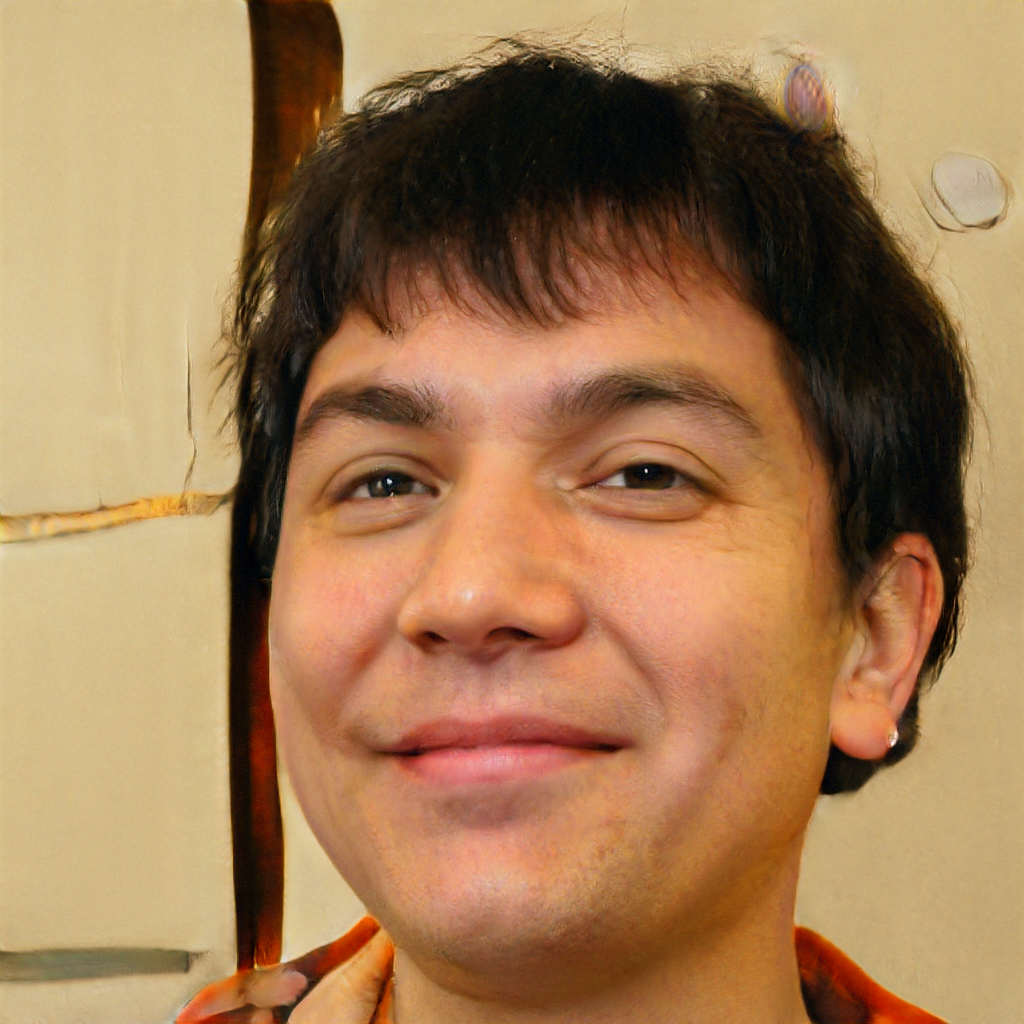
\includegraphics[width=.3\linewidth]{img/gen/1.png} &
      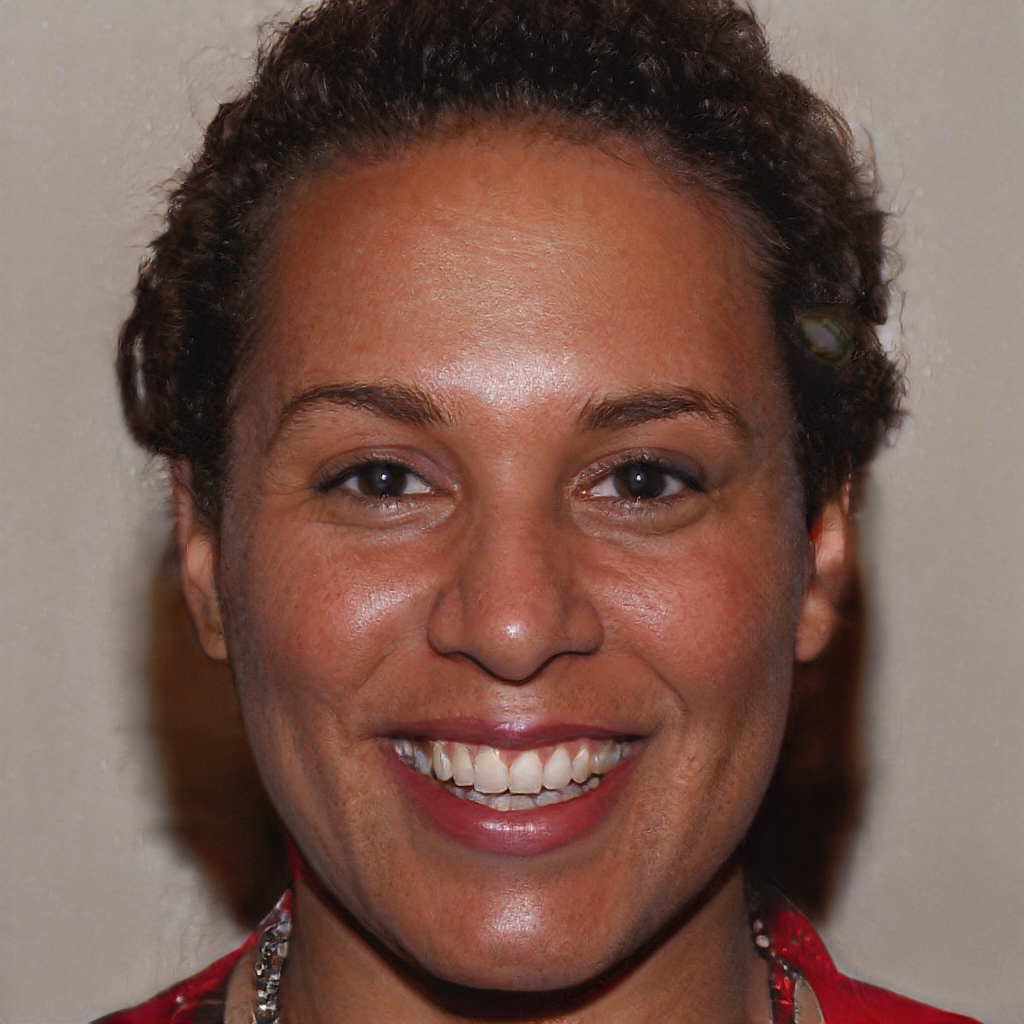
\includegraphics[width=.3\linewidth]{img/gen/2.png} &
      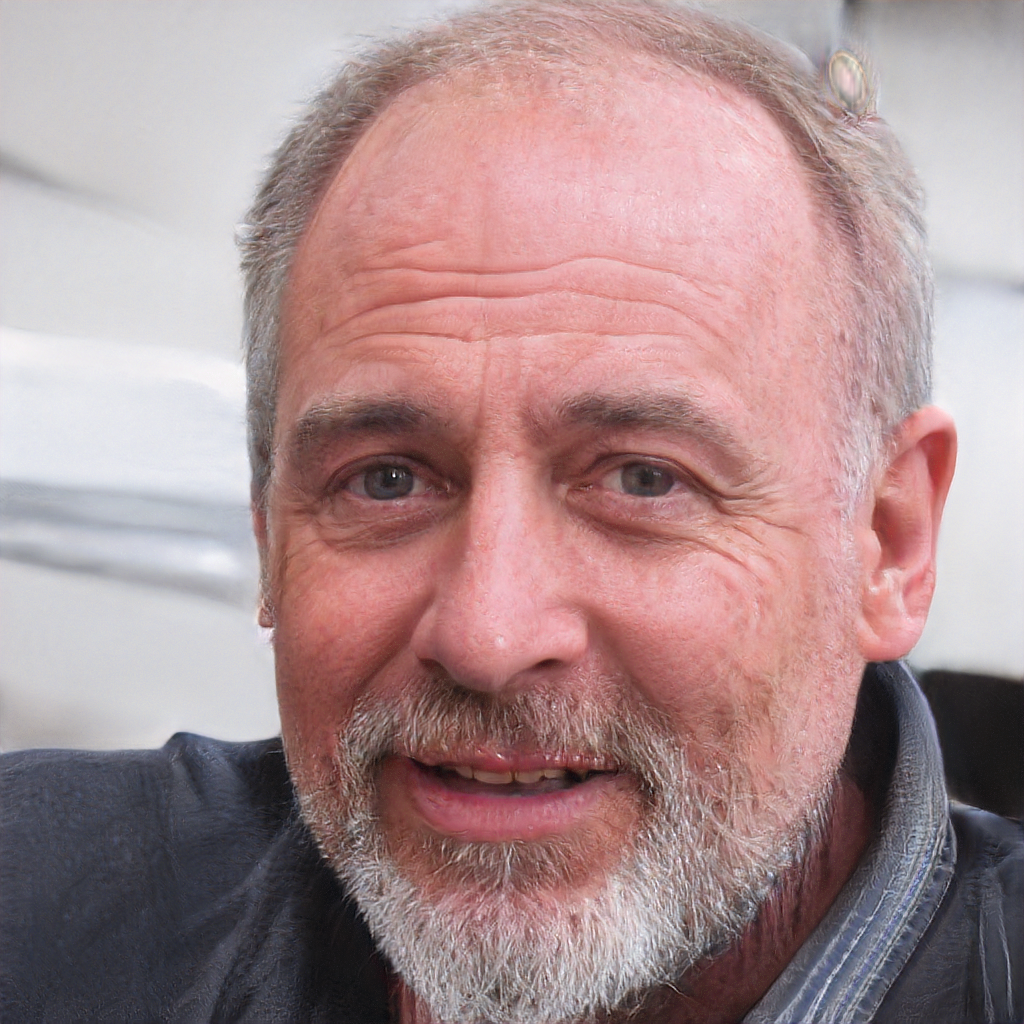
\includegraphics[width=.3\linewidth]{img/gen/3.png} \\
      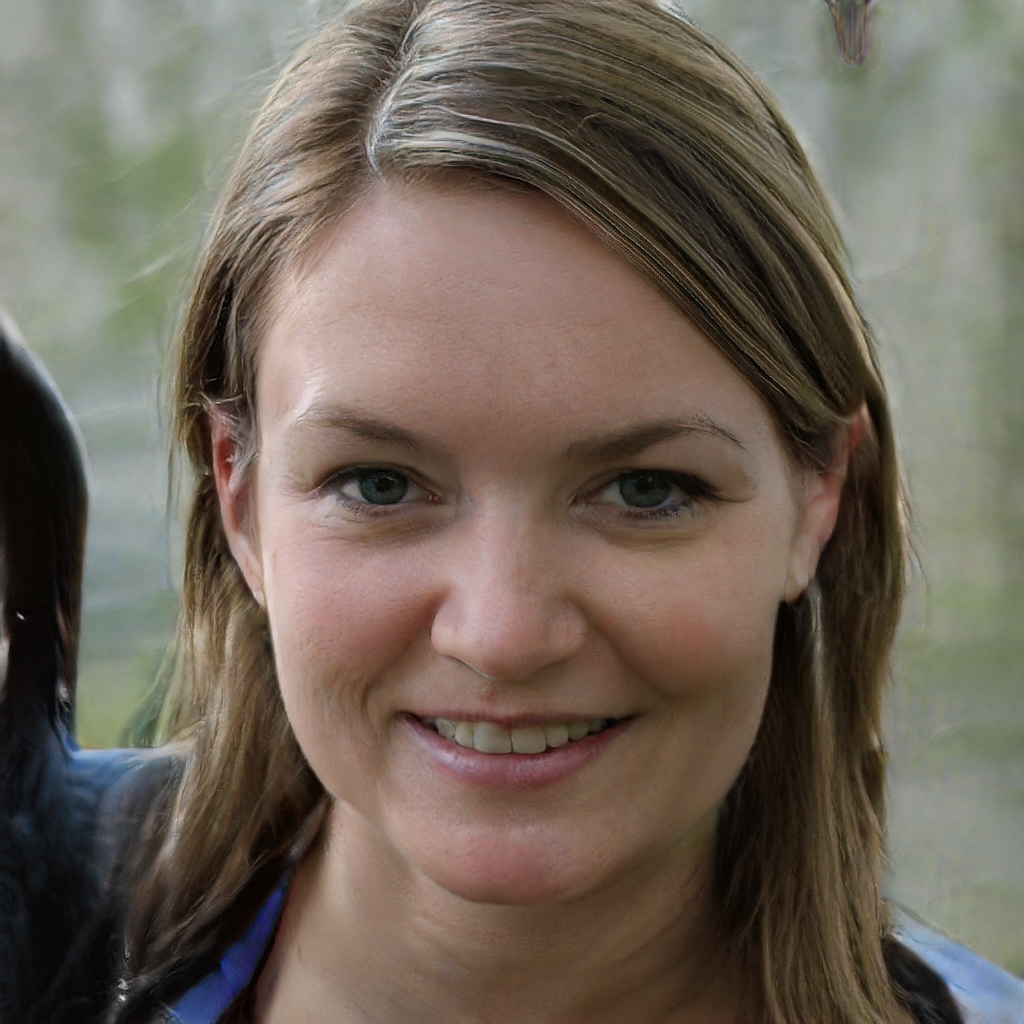
\includegraphics[width=.3\linewidth]{img/gen/4.png} &
      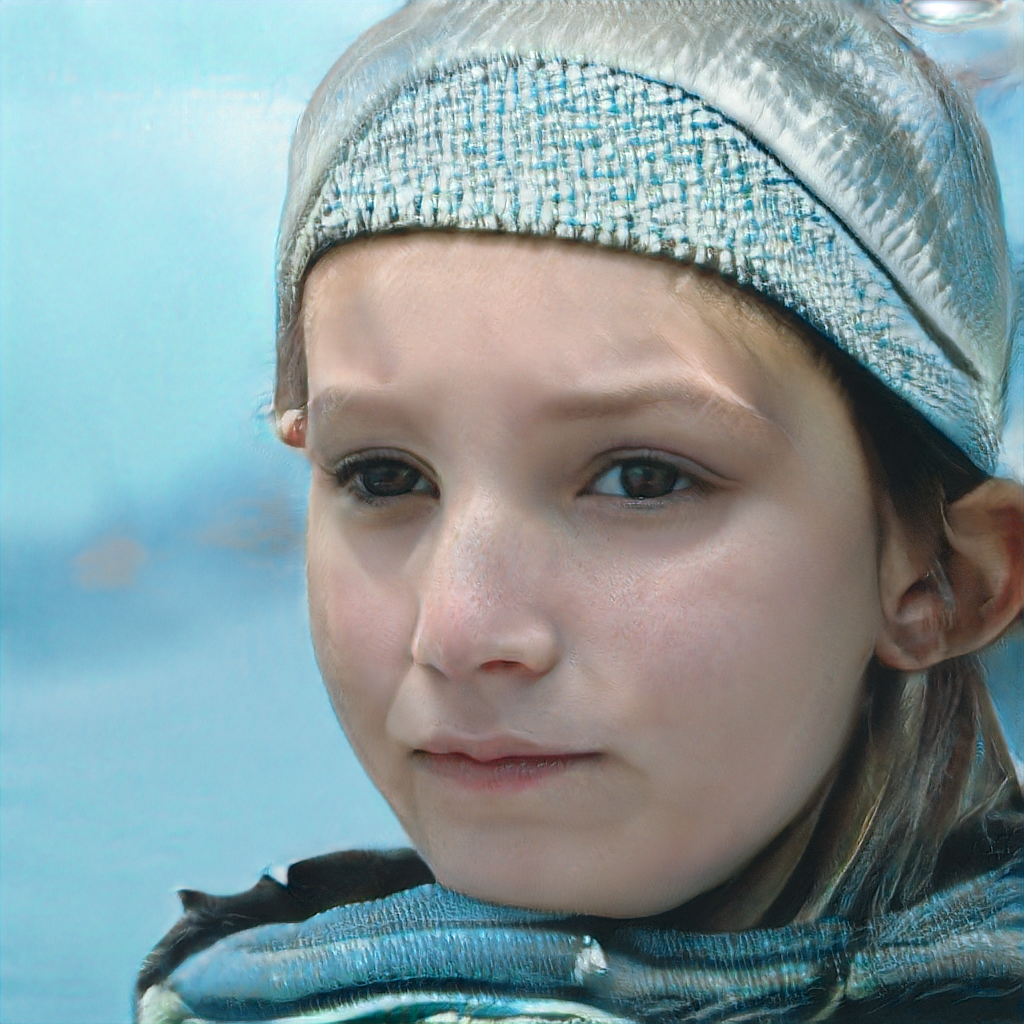
\includegraphics[width=.3\linewidth]{img/gen/5.png} &
      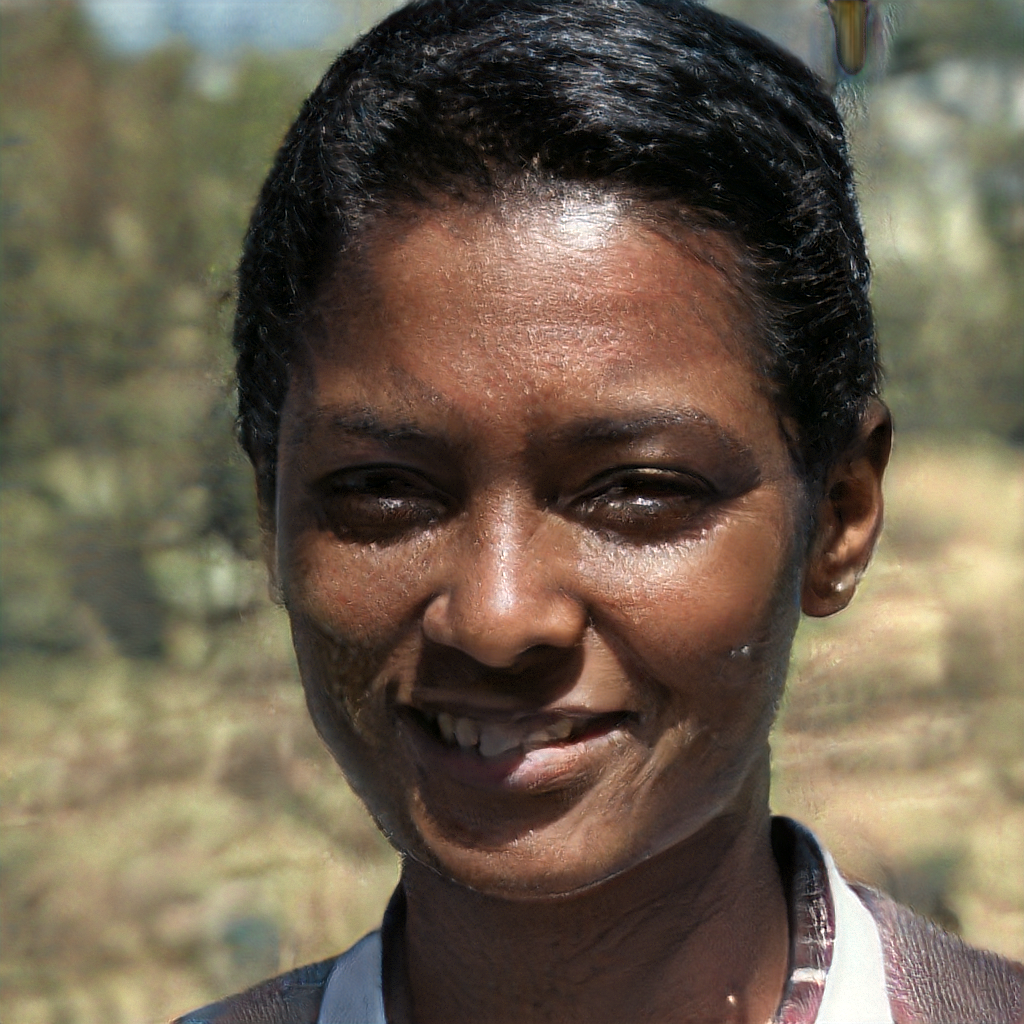
\includegraphics[width=.3\linewidth]{img/gen/6.png} \\
      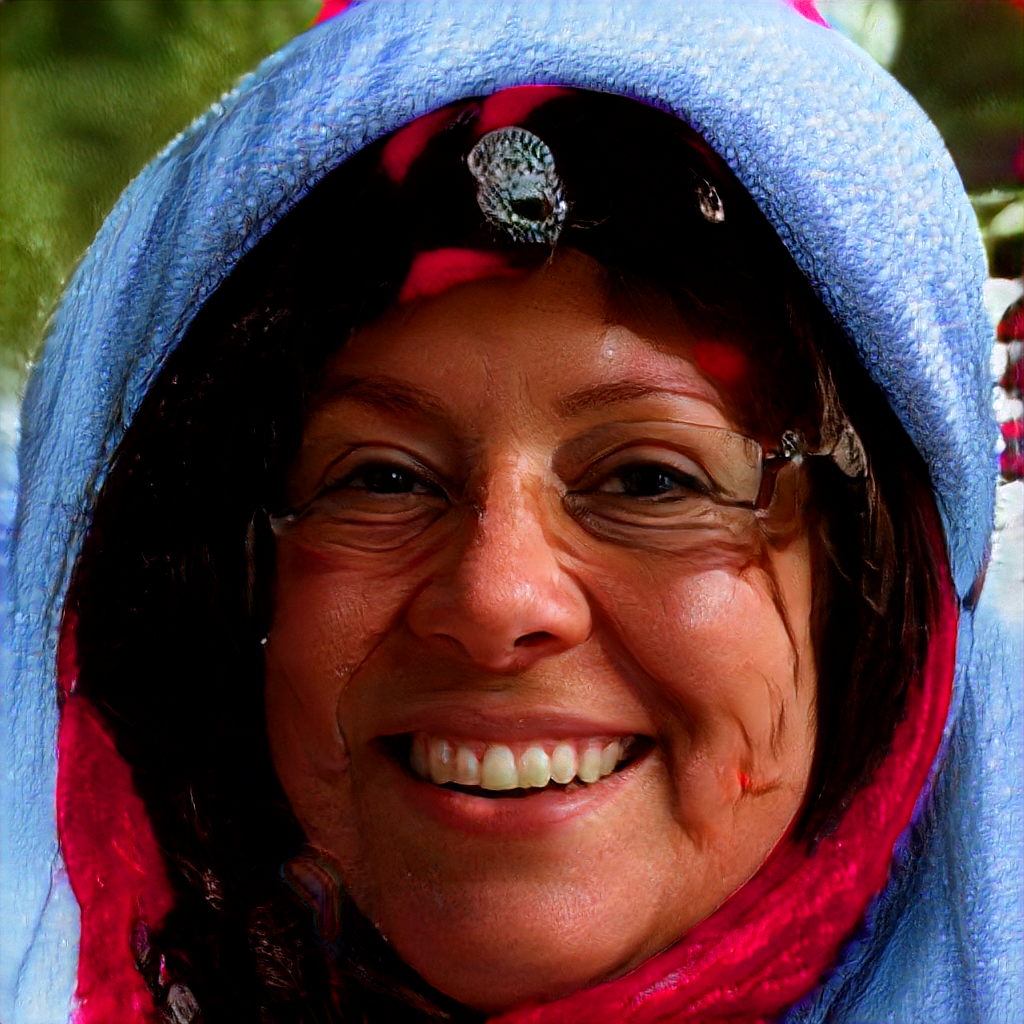
\includegraphics[width=.3\linewidth]{img/gen/7.png} &
      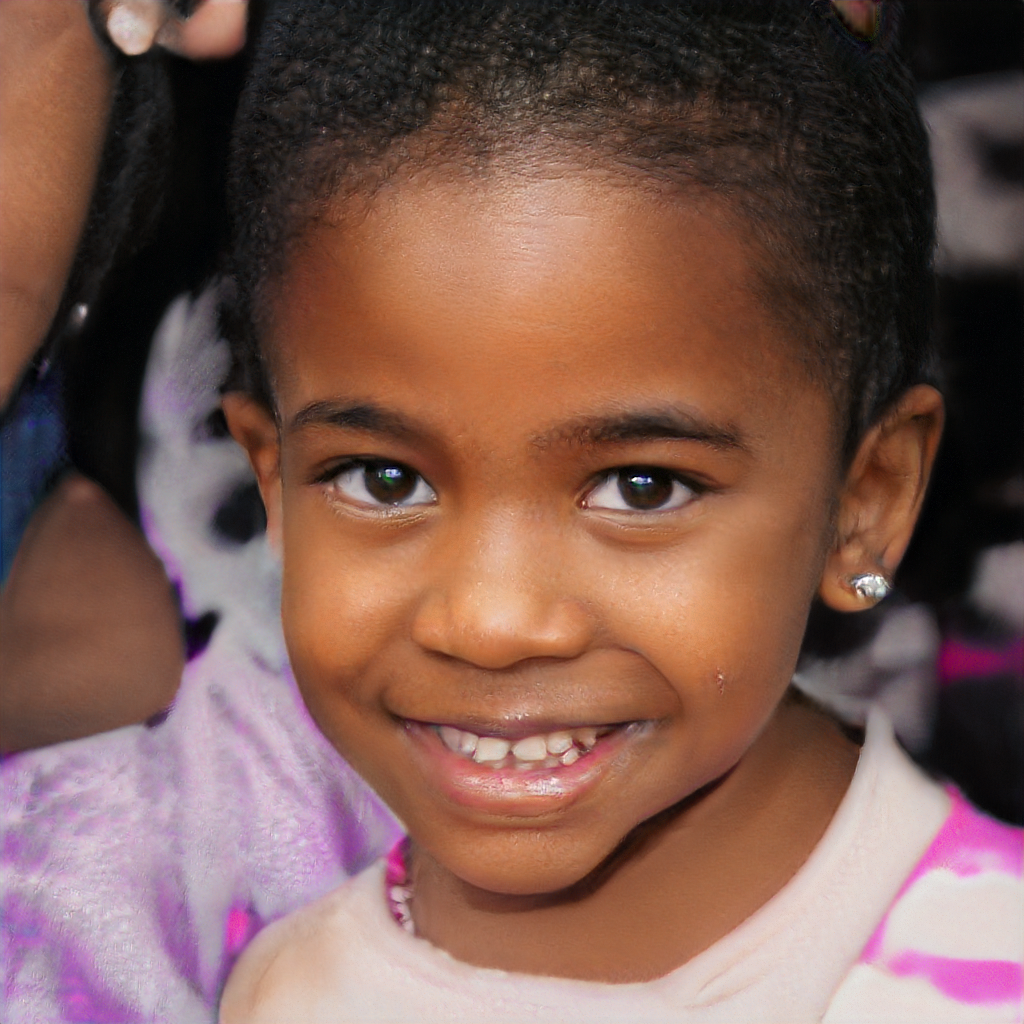
\includegraphics[width=.3\linewidth]{img/gen/8.png} &
      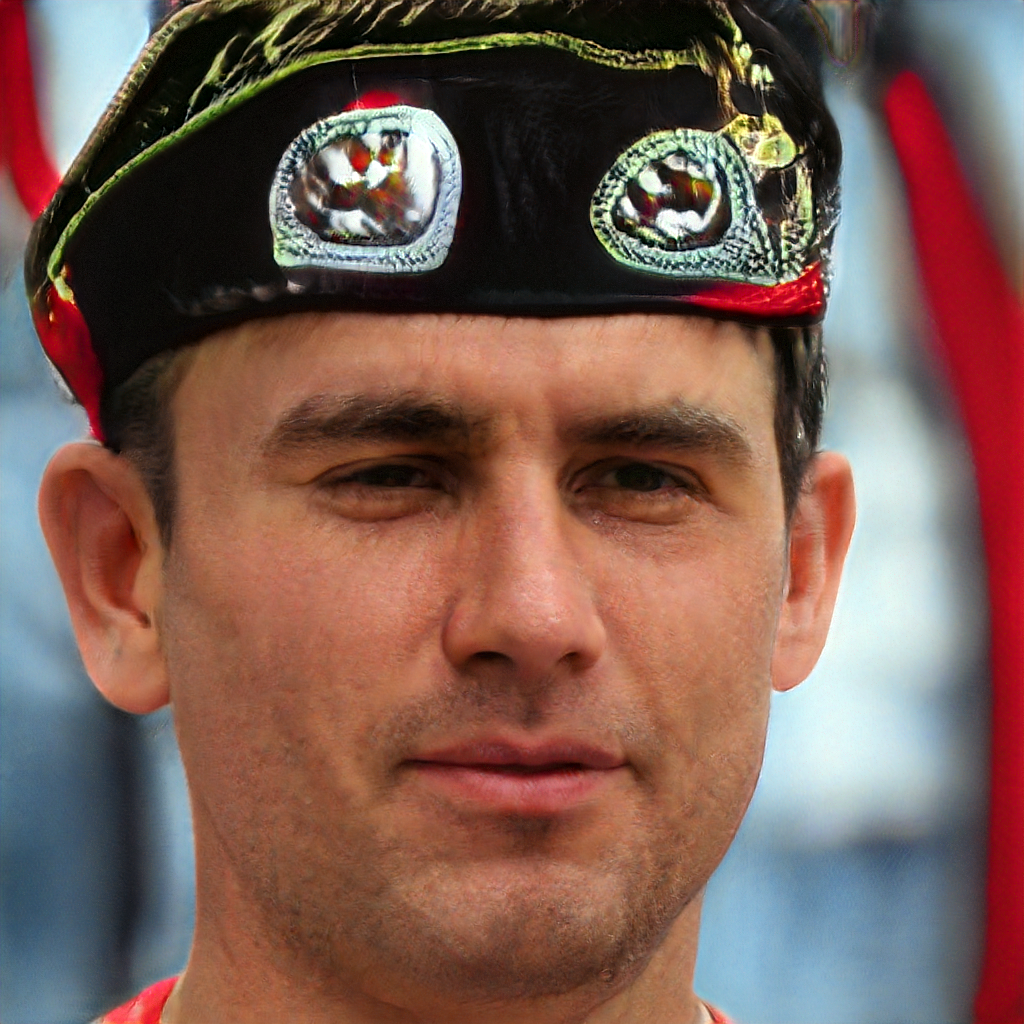
\includegraphics[width=.3\linewidth]{img/gen/9.png} \\
    \end{tabular}
    \end{center}
    \caption{{\bf Przykłady działania generatora twarzy.}}
    \label{fig:generator_twarzy}
    \end{figure}




  \subsection{Zbiory danych}
  \begin{table}[H]
  \begin{center}
  \begin{tabular}{ccccc}
  \hline
  Zbiór danych  & \# osób   &   \# zdjęć  &   \# zdjęć na osobę   &   aligned \\
  \hline
  MS1M-DeepGlint \cite{glintweb}   & 87K  & 3.9M & ?/44.8/? & Tak \\
  \hline
  \hline
  VGGFace2-test-train   & 500 & 163.3K & ?/361/? & Nie  \\
  StyleGAN-0.7   & 1M & 1M & 1 & Nie  \\
  \hline
  \hline
  VGGFace2-test-test    & 500 & 18.1K & ?/361/? & Nie  \\
  \hline
  \end{tabular}
  \end{center}
  \caption{\textbf{Zbiory danych} MS1M-DeepGlint posłuży do wytrenowania ekstraktora cech, a VGGFace2-test po podzieleniu do treningu oraz testowania treningu FL.} \label{table:dataset-FL}
  \vspace{-4mm}
  \end{table}


  \subsection{Eksperymenty}
  \subsubsection{Metoda pre-treningu modelu}
  \subsubsection{Online Hard sample mining}

\newpage
\section[summary]{Podsumowanie}\label{sec:summary}


%--------------------------------------------
% Literatura
%--------------------------------------------
\newpage
\printbibliography{}

%--------------------------------------------
% Spisy (opcjonalne)
%--------------------------------------------
\newpage

% Wykaz symboli i skrótów.
% Pamiętaj, żeby posortować symbole alfabetycznie
% we własnym zakresie. Ponieważ mało kto używa takiego wykazu, 
% uznałem, że robienie automatycznie sortowanej listy
% na poziomie LaTeXa to za duży overkill. 
% Jest tylko proste i oczywiste makro \acronym, 
% które dodaje postawowe formatowanie. 
% //AB
\vspace{0.8cm}
\section*{Wykaz symboli i skrótów}
\acronym{EiTI}{Wydział Elektroniki i Technik Informacyjnych}
\acronym{PW}{Politechnika Warszawska}

% \listoffigures              % Spis obrazków. 
% \vspace{1cm}                % vertical space
% \listoftables               % Spis tabel. 
% \vspace{1cm}                % vertical space
% \listofappendices{}           % Spis załączników

% Załączniki
% \appendix

% \newpage
% \newappendix{Nazwa załącznika 1}
% \lipsum[1]

% \newpage
% \newappendix{Nazwa załącznika 2}
% \lipsum[1]

% Używając powyższych spisów jako szablonu,
% możesz tu dodać swój własny wykaz bądź listę, 
% np. spis algorytmów. 

\end{document} % Dobranoc. 

